\documentclass{article}

% ─────────────────────────── PACKAGES ────────────────────────────
\usepackage{times}
\usepackage{geometry}
\geometry{a4paper,left=0.6cm,right=0.7cm,top=1cm,bottom=1cm,columnsep=0.8cm}

\usepackage{fontawesome}
\usepackage[hidelinks]{hyperref}
\usepackage{paracol}
\usepackage{tikz}
\usepackage{tabularx}
\usepackage{xcolor}
\usepackage{enumitem}


\definecolor{maincolor}{HTML}{ffffff}
\definecolor{seccolor}{HTML}{0b1f3b}
\definecolor{gray}{HTML}{8c94a9}
\definecolor{sidetext}{HTML}{59cee5}
\definecolor{Green}{HTML}{2caf00}
\definecolor{lightgray}{HTML}{D3D3D3}
%\definecolor{maincolor}{HTML}{2AAEE7}

\newcolumntype{Y}{>{\RaggedRight\arraybackslash}X}
\setlist[itemize]{itemsep=-2pt,topsep=0pt,leftmargin=*}
\renewcommand{\labelitemi}{\textcolor{black}{\footnotesize$\bullet$}}
%
\setlength{\parindent}{0pt}

% titre de section
\newcommand{\cvsection}[1]{%
  \par\bigskip
  \begin{tabular}{@{}p{\linewidth}}
  \textbf{\Large #1}\\[3pt]\hline
  \end{tabular}\medskip}

\newcommand*{\ClipSep}{0.4cm}

\setlength{\columnseprule}{0.4pt}        % épaisseur du trait
\setlength{\columnsep}{0.8cm}            % (facultatif : rappel de l’écart)
\def\columnseprulecolor{\color{lightgray}}% couleur du trait
% ─────────────────────────── DOCUMENT ────────────────────────────
\begin{document}\pagestyle{empty}
\columnratio{0.7}\begin{paracol}{2}

%%%%%%%%%%%%%%%%%%%%%%%%%%%%%%%%%%%%%%%%%%%%%%%%%%%%%%%%%%%%%%%%%%%
% Colonne gauche (70 %)
%%%%%%%%%%%%%%%%%%%%%%%%%%%%%%%%%%%%%%%%%%%%%%%%%%%%%%%%%%%%%%%%%%%

{\LARGE\textbf{Judikael MOUROUVIN}}

\bigskip
{\color{sidetext}\Large\textbf{Alternant en marketing digital \& support informatique}}

\medskip
\begin{tabular}{@{}cp{0.4\linewidth}cp{0.4\linewidth}}
  \color{sidetext}\faEnvelope & \href{mailto:jkmou971@gmail.com}{jkmou971@gmail.com} &
  \color{sidetext}\faMapMarker & Route de COCOYER\;97190 GOSIER\\[6pt]
  \color{sidetext}\faPhone & \href{tel:+590 0690 91 14 48}{+590 0690 91 14 48} &
  \color{sidetext}\faLinkedin & \href{}{}
\end{tabular}

\cvsection{EXPERIENCE}

\colorbox{maincolor}{%
  \begin{minipage}{\linewidth}
    \textbf{Alternant en Marketing Digital} \\ Mairie du Gosier, DSI \\ 2023-2024
    \begin{itemize}
      \item Géré divers projets numériques municipaux, assurant leur déploiement efficace. \item Analysé les besoins des agents et mis en place des solutions adaptées pour améliorer la productivité. \item Assuré support et formations tout en contribuant à la stratégie de marketing digital de la collectivité.
    \end{itemize}
  \end{minipage}}

\vspace{3mm}


\colorbox{maincolor}{%
  \begin{minipage}{\linewidth}
    \textbf{Animateur de la zone informatique} \\ POLE EMPLOI, Gosier \\ 2022-2023
    \begin{itemize}
      \item Fournit assistance et support technique quotidien aux utilisateurs internes et externes. \item Configuré et entretenu les postes de travail afin de garantir leur disponibilité. \item Diagnostiqué et résolu les incidents informatiques pour réduire les interruptions de service.
    \end{itemize}
  \end{minipage}}

\vspace{3mm}


\colorbox{maincolor}{%
  \begin{minipage}{\linewidth}
    \textbf{Stagiaire Informaticien} \\ NUMERIKA, Baie Mahault \\ 2020-2021
    \begin{itemize}
      \item Installé, configuré et maintenu les équipements informatiques de l’entreprise. \item Assuré un support technique réactif aux équipes pour garantir la continuité des opérations.
    \end{itemize}
  \end{minipage}}      %← généré dynamiquement (blocs colorbox)

\cvsection{EDUCATION}

    \begin{tabularx}{\linewidth}{@{}c X@{}}
    \textcolor{sidetext}{\faGraduationCap} &
    \textbf{Bachelor Marketing Digital} \\
    & CFA IUTS \\
    & \begin{itemize}[leftmargin=*]
  \item Étude des stratégies de marketing en ligne, SEO/SEA et médias sociaux. \item Analyse de performance digitale et gestion de campagnes multicanales.
\end{itemize} \\
    & \textit{2023-2024}
    \end{tabularx}
    

\vspace{3mm}


    \begin{tabularx}{\linewidth}{@{}c X@{}}
    \textcolor{sidetext}{\faGraduationCap} &
    \textbf{BTS Système Numérique option Informatique et Réseaux} \\
    & Lycée de Chevalier Saint Georges, Abymes \\
    & \begin{itemize}[leftmargin=*]
  \item Apprentissage de l’architecture réseau, protocoles et cybersécurité. \item Mise en pratique de la maintenance matérielle et logicielle des systèmes informatiques.
\end{itemize} \\
    & \textit{2019-2021}
    \end{tabularx}
              %← idem



%%%%%%%%%%%%%%%%%%%%%%%%%%%%%%%%%%%%%%%%%%%%%%%%%%%%%%%%%%%%%%%%%%%
% Colonne droite (30 %)
%%%%%%%%%%%%%%%%%%%%%%%%%%%%%%%%%%%%%%%%%%%%%%%%%%%%%%%%%%%%%%%%%%%
\switchcolumn
\centering
\begin{tikzpicture}
  \clip (0,0) circle (1.5cm) node[anchor=center]
        {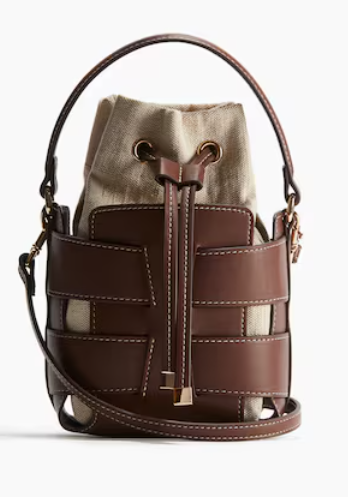
\includegraphics[width=3cm]{74a5db6206ef405ebd3598f8977bae72.png}};
\end{tikzpicture}


\cvsection{SUMMARY}
Passionné par l’informatique et le marketing digital, j’ai développé une solide expertise en maintenance, diagnostic et accompagnement des utilisateurs. Mon année d’alternance à la DSI de la Mairie du Gosier m’a permis de mener des projets numériques tout en renforçant la stratégie de communication en ligne. Rigoureux et orienté résultat, je sais analyser les besoins, proposer des solutions adaptées et former les collaborateurs. Je souhaite désormais mettre ces compétences au service de nouveaux défis à temps plein.

\cvsection{SKILLS}
\begin{itemize}[leftmargin=*]
\item Administration
\item Réseaux
\item Support
\item Diagnostic
\item Maintenance
\item Marketing
\item Configuration\end{itemize}

\cvsection{LANGUAGES}
\begin{itemize}[leftmargin=*]
\item English - \textcolor{gray}{}
\item Espagnol - \textcolor{gray}{}\end{itemize}

\cvsection{INTERESTS}
\begin{itemize}[leftmargin=*]
\item Lecture \& veille technologique
\item Randonnée / sports outdoor
\item Voyages \& découverte culturelle
\end{itemize}

\end{paracol}
\end{document}
